% !TEX root = ../paper.tex
\documentclass[../paper.tex]{subfiles}
\begin{document}


В рамках данной работы было написано програмное обеспечение для работы с ультразвуковым стетоскопом. Были разработаны программы под 2 разных АЦП: ЗАО "Руднев-Шиляев" ЛА-н10-12USB и Arduino Due. Также была написана программа для вычисления быстрого преобразования Фурье на удаленном высокопроизводительном сервере с помощью технологии NVidia CUDA.

Ниже приводятся описания программ для работы с двумя разными АЦП а также описание программы, запускаемой на CUDA-сервере.

\subsection{Програмное обеспечение для ЛА-н10-12USB}

Програмное обеспечение написано на языке C\# для платформы Windows.

В функционал програмного обеспечения входит:
\begin{itemize}
  \item Получение сигнала от АЦП ЛА-н10-12USB
  \item Отображение сигнала в реальном времени на экране в виде графика
  \item Отображение спектра сигнала полученного в результате быстрого преобразования Фурье
  \item Отображение скользящего среднего сигнала
  \item Возможность записи сигнала на жесткий диск для последующей обработки
\end{itemize}

\subsubsection{Инструкция по установке ПО}
\begin{itemize}
  \item Скачать драйверы для АЦП ЛА-н10-12USB по ссылке:\cite{rudshel-drivers}\\ 
  \item Запустить и установить файл RShUSBDriver\_XP\_Vista\_7\_8\_x86\_x64\_SDK2\_2.0.x.y.exe (драйверы для USB устройств)
  \item Запустить и установить файл RshSDKSetup\_2.0.x.y.exe (средства разработки ПО (SDK))
  \item Скачать проект для работы со стетоскопом по ссылке \cite{app-rudshel}
  \item Скомпилировать проект с помощью IDE Microsoft Visual Studio.
\end{itemize}

\subsubsection{Описание интерфейса пользователя ПО} 
\begin{figure}[H]
\centering
% 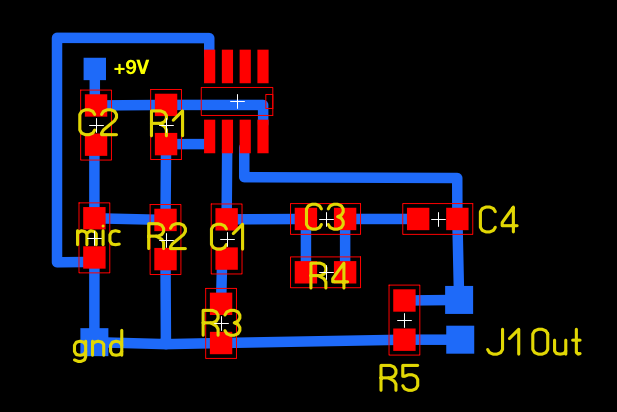
\includegraphics[width=14cm]{sprint-layout-circuit.png}
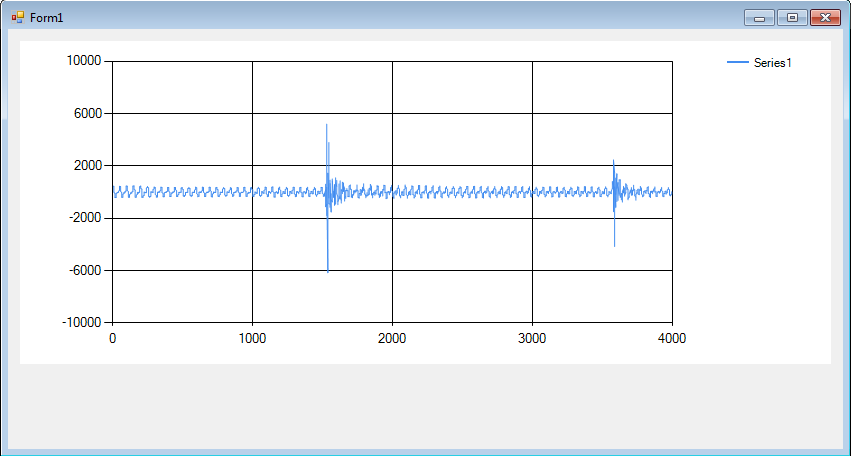
\includegraphics[width=\textwidth]{images/screenshot.png}
\caption{Скриншот работы программы}
\end{figure}
В центре находится график сигнала с АЦП. Справа находится кнопка старт/стоп, которая управлет запуском и остановкой сбора сигнала с АЦП. Справа вверху есть числовое поле, которое отвечает за количество точек по горизонтальной оси на графике. Кнопки "+/-" Отвечают за увеличение и уменьшение размеров графика (zoom).

\subsubsection{Описание кода программы}
В начале программы задаются параметры размера буффера и частоты дискретизации (\lstinline|RATE|).
\begin{lstlisting}
const uint   BSIZE              = 524288; // размер_буффера
const double RATE               = 8.0e+7;
\end{lstlisting}


Далее при нажатии пользователем на кнопку старт, программа начинает инициализацию АЦП. Она проверяет подключено ли устройство, проверяет его работоспособность и начинает сбор данных.

За инициализацию отвечают следующие строчки в коде:

\begin{lstlisting}
//========================== INITIALISATION ================        
st = device.EstablishDriverConnection(BOARD_NAME); //load and connect to device's library
if (st != RSH_API.SUCCESS) SayGoodBye(st);
st  = device.Connect(1); // connecting to device
if (st != RSH_API.SUCCESS) SayGoodBye(st);
p.startType           = (uint)RshInitMemory.StartTypeBit.Program;  
p.bufferSize          = BSIZE; // Internal buffer block sizr
p.frequency           = RATE;  // Sampling rate
p.channels[0].control = (uint)RshChannel.ControlBit.Used;  // make 0 channel active
p.channels[0].gain    = 10; // gain coefficient for 0 channel
[1, 2, 5, 10] ~ [+-0.2V, +- 0.4V, +-1V, +- 2V]
st = device.Init(p); // Initialisaton 
if (st != RSH_API.SUCCESS) SayGoodBye(st);
\end{lstlisting}


Далее программа ждет пока пользователь нажмет кнопку старт. При нажатии на кнопку старт вызывается функция \lstinline|button1_Click|, которая в свою очередь запускает новый процесс \lstinline|backgroundWorker1_DoWork|. Этот процесс собирает данные с АЦП в бесконечном цикле пока пользователь не нажмет на кнопку стоп. Он записывает значения с АЦП в структуру данных очередь, доступ к которой имеет UI-процесс (процесс, отвечающий за отображение и обработку элементов пользовательского интерфейса). По мере обновления данных UI процесс обновляет график.

За старт, сбор данных и остановку АЦП отвечает следующий блок кода: 

\begin{lstlisting}
double[] buffer = new double[p.bufferSize]; // buffer from adc
uint waitTime = 100000; // wait time (in miliseconds) until buffer overlflow // default = 100000
while (getting_data)
{
    stopwatch.Restart();

    st = device.Start();
    if (st != RSH_API.SUCCESS) SayGoodBye(st);

    st = device.Get(RSH_GET.WAIT_BUFFER_READY_EVENT, ref waitTime);
    if (st != RSH_API.SUCCESS) SayGoodBye(st);

    st = device.GetData(buffer); // very big amount of data
    if (st != RSH_API.SUCCESS) SayGoodBye(st);

    device.Stop();

    // Queue Dequeue and Enqueue implementation with arrays
    double[] values_to_draw_copy = (double[])values_to_draw.Clone();
    for (int i = 0; i < x_axis_points - r_buffer_size; i++) 
        values_to_draw[i] = values_to_draw_copy[r_buffer_size + i];

    for (int i = 0; i < r_buffer_size; i++)
        values_to_draw[x_axis_points - r_buffer_size + i] = 
        buffer[BSIZE / r_buffer_size * i];

    stopwatch.Stop();
    Console.WriteLine("GetData() time:\t" + 
    stopwatch.ElapsedMilliseconds + "ms");
} 
\end{lstlisting}

Также процесс backgroundWorker замеряет время каждого цикла сбора данных. (stopwatch.Restart() и stopwatch.Stop()) Это время процесс пользовательского интерфейса выводит на экран.

\subsubsection{Измерение времени работы АЦП}
Как уже было сказано выше, в зависимости от различных значений размера буффера и частоты дискретизации у АЦП уходит различное время на перезапуск и сбор данных. Эти вычисления производились при помощи стандартной функции-секундомера из стандартной библиотеки C\#.

\subsubsection{Паралельные вычисления в программе}
В программе используются паралельные вычисления. Присутсвуют два потока. Один поток работает с АЦП: принимает данные и записывает во временный буфер. Другой поток - отрисовывает данные из буффера на графике а также обрабатывает команды пользователя. 

Паралельные вычисления используются из-за необходимости непрерывно получать данные с АЦП, чтобы избежать потери данных. Также, если не использовать паралельные вычисления, то приложение может не реагировать на команды пользователя из за того что процессор будет занят работой с АЦП.

\subsection{Програмное обеспечение для Arduino Due}
Програмное обеспечение для микроконтроллера Arduino Due состоит из программы, запускаемой на Arduino и программы, запускаемой на компьютере. 
Возможности програмного обеспечения:
\begin{enumerate}
  \item Прием сигнала от АЦП Arduino через Native-USB порт
  \item Визуализация сигнала в реальном времени
  \item Запись на диск в бинарный файл
  \item Отправка записаного сигнала на CUDA-сервер для вычисления быстрого преобраззования Фурье.
  \item Возможность посчитать быстрое преобраззование Фурье локально
\end{enumerate}

\begin{figure}[H]
\centering
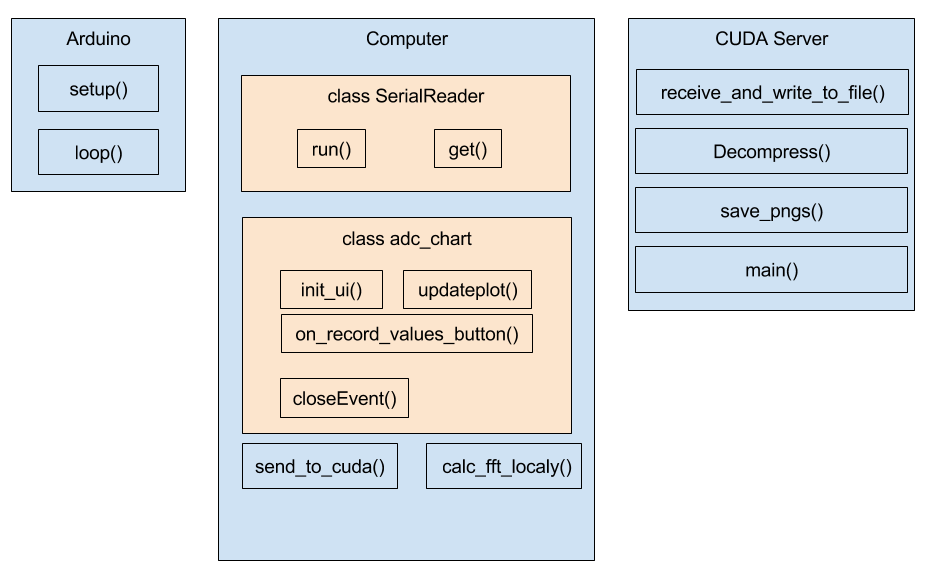
\includegraphics[width=\textwidth]{images/soft-blueprint.png}
\caption{Диаграмма классов ПО для Arduino Due}
\end{figure}

\subsubsection{Программа для запуска на Arduino}
Для того, чтобы ардуино работало в нужном режиме, на него нужно записать следующую программу:
% \begin{lstinlineatim}
\begin{lstlisting}
#undef HID_ENABLED
volatile int bufn,obufn;
uint16_t buf[4][256];   // 4 buffers of 256 readings

void ADC_Handler(){     // move DMA pointers to next buffer
  int f=ADC->ADC_ISR;
  if (f&(1<<27)){
   bufn=(bufn+1)&3;
   ADC->ADC_RNPR=(uint32_t)buf[bufn];
   ADC->ADC_RNCR=256;
  } 
}

void setup(){
  SerialUSB.begin(0);
  while(!SerialUSB);
  pmc_enable_periph_clk(ID_ADC);
  adc_init(ADC, SystemCoreClock, ADC_FREQ_MAX, ADC_STARTUP_FAST);
  ADC->ADC_MR |=0x80; // free running

  ADC->ADC_CHER=0x80; 

  NVIC_EnableIRQ(ADC_IRQn);
  ADC->ADC_IDR=~(1<<27);
  ADC->ADC_IER=1<<27;
  ADC->ADC_RPR=(uint32_t)buf[0];   // DMA buffer
  ADC->ADC_RCR=256;
  ADC->ADC_RNPR=(uint32_t)buf[1]; // next DMA buffer
  ADC->ADC_RNCR=256;
  bufn=obufn=1;
  ADC->ADC_PTCR=1;
  ADC->ADC_CR=2;
}

void loop(){
  while(obufn==bufn); // wait for buffer to be full
  SerialUSB.write((uint8_t *)buf[obufn],512); // send it - 512 bytes
  = 256 uint16_t
  obufn=(obufn+1)&3;    
}
% \end{lstinlineatim}
\end{lstlisting}


Данный код запускает АЦП в так называемом Free Running Mode. Это самый быстрый режим работы данного АЦП. Его особенность заключается в том, что нет необходимости вручную собирать данные через определенное количество времени. Программа пользователя запускает только первый сбор данных, а дальше АЦП сам автоматически начинает преобразование сразу как только закончилось предыдущее. Таким образом не возникает простоев АЦП и не теряются данные.

Также здесь используется прямой доступ к памяти микроконтроллера AT91S-AM3X8E. (Direct Memory Access / DMA). Этот режим позволяет обращаться напрямую к памяти микроконтроллера, таким образом не отнимая процессорное время самого микроконтроллера. Процессор не прерывается на обработку запроса к памяти и постоянно занят сбором данных с АЦП. Это позволяет приблизится к максимальной частоте дискретизации.

Чтобы установить данное ПО на Arduino Due, необходимо скачать Arduino IDE с официального сайта Arduino\cite{arduino-ide}

Устройсво нужно подключить к компьютеру через USB порт. Данное устройство имеет 2 USB порта: программируемый и native. Чтобы записать программу нужно подключаться через програмируемый.

В Arduino IDE в меню Tools - Board нужно выбрать "Arduino Due (Programming Port)" как показано на скриншоте ниже.
\begin{figure}[H]
\centering
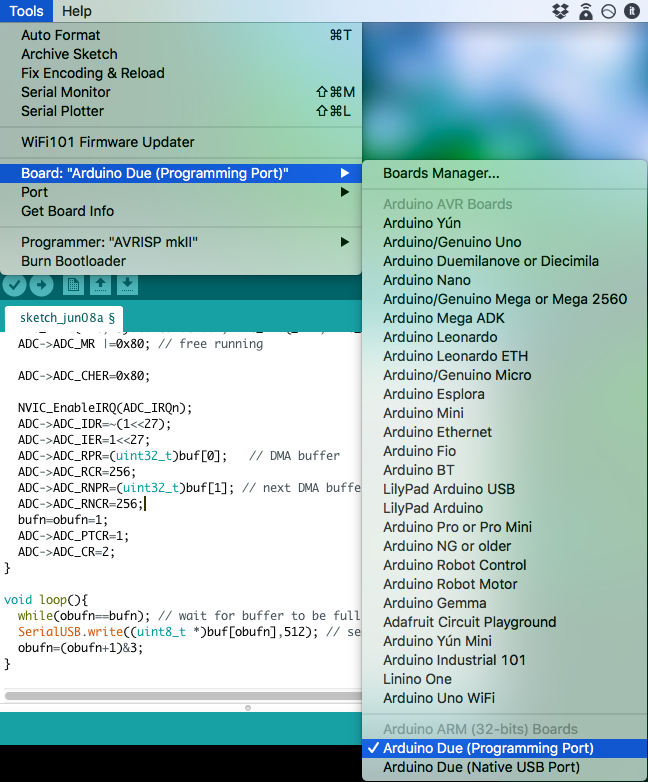
\includegraphics[width=16cm]{images/ard-board-select.png}
\end{figure}

В главное окно программы нужно вставить код, приведенный выше и нажать кнопку Upload. После этого программа будет успешно записана на микроконтроллер.

\subsubsection{Программа для запуска на компьютере}
Данное ПО написано на языке Python и может быть запущено на любой операционной системе. Используются библиотеки PyQtgraph, PyQt, numpy, matplotlob и pyserial. Для запуска программы необходимо установить эти библиотеки:
\begin{enumerate}
  \item Скачать и установить последнюю версию python c официального сайта\cite{python}
  \item открыть командную строку и установить необходимые библиотеки с помощью комманд:
  \item sudo pip install pyqtgraph
  \item pip install pyqt5
  \item pip install numpy
  \item pip install matplotlib
  \item pip install pyserial
  \item скачать саму программу для работы с ацп по ссылке: \cite{app}
\end{enumerate}

Даллее в коммандной строке необходимо перейти в директорию, где находится скачанная программа \lstinline|app.py|. Теперь нужно подключить устройство к компьютеру через Native-USB порт и запустить программу с помощью команды:

\lstinline|python app.py|

При запуске программы можно указывать параметры децимации (downsampling). Децимация позволяет отрисовывать на графике не все значения с АЦП, а в N раз меньше. Это позволяет увеличить скорость отрисовки (Более высокое значение FPS (frames per second, количество кадров в секунду), но при этом теряется точность сигнала, можно не увидеть очень высоие частоты на графике. Значение децимации задается с помощью аргумента \lstinline|-d|. Допустим, команда

\lstinline|python app.py -d 100|

запустит программу со значением параметра децимации=100.

\begin{figure}[H]
\centering
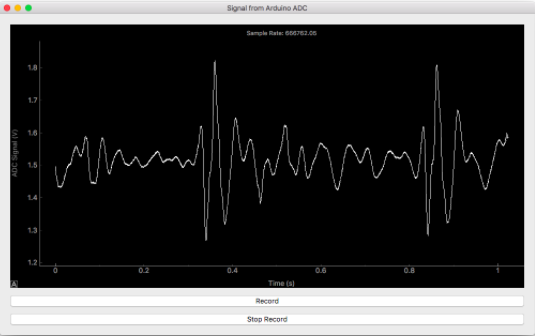
\includegraphics[width=\textwidth]{images/heart}
\caption{Скриншот работы программы, прослушивается сердце. Сигнал отображается с децимацией=100. Частота дискретизации 666кГц.}
\end{figure}

\begin{figure}[H]
\centering
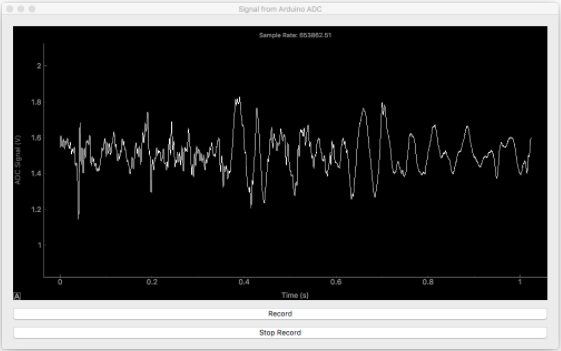
\includegraphics[width=\textwidth]{images/lungs}
\caption{Скриншот работы программы, прослушиваются легкие. Сигнал отображается с децимацией=100. Частота дискретизации 666кГц.}
\end{figure}

Для записи данных в файл и отправки их на сервер нужно выбрать сколько значений записывать и нажать кнопку Record Values.

Основные компоненты программы:
\begin{itemize}
  \item Класс \lstinline|SerialReader| - принимает данные с ацп через serial порт. В этом классе есть 2 основных метода: метод \lstinline|run()|, который в бесконечном цикле собирает данные с АЦП и, если нажата кнопка записи, записывает данные в файл. Метод \lstinline|get(num, downsample=1| - возвращает num последних значений с ацп. Этот метод использует второй класс \lstinline|adc_chart|
  \item Класс \lstinline|adc_chart| - работает с интерфейсом пользователя. Основные методы: 
    \begin{itemize}
      \item \lstinline|init_ui| - инициализация пользовательского интерфейса
      \item \lstinline|updateplot| - метод получает последние значения с АЦП и отрисовывает их на графике
      \item \lstinline|on_record_values_button| - обработка кнопки записи сигнала.
      \item \lstinline|closeEvent| - обработка закрытия окна программы. Завершает все запущенные процессы.
    \end{itemize}
  \item \lstinline|send_to_cuda| - метод вызываемый, когда завершена запись данных. Отправляет данные на CUDA-сервер.
  \item \lstinline|calc_fft_localy| - метод позволяющий посчитать быстрое преобразование Фурье на локальном компьютере, без отправки на сервер. Для вычисления и отрисовки используются библиотеки Numpy и Matplotlib.
\end{itemize}

\begin{figure}[H]
\centering
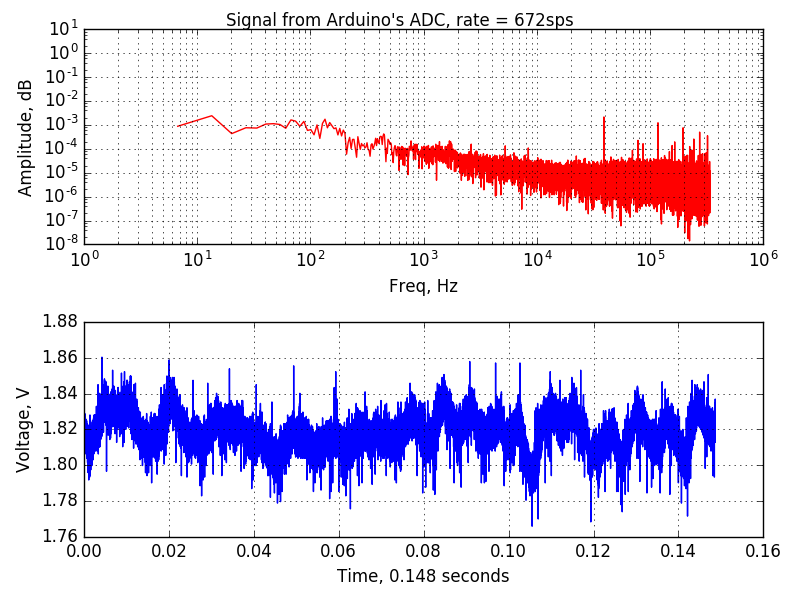
\includegraphics[width=\textwidth]{images/fft-local}
\caption{Изображения, получающиеся при локальном преобразовании Фурье}
\end{figure}

\subsection{Програмное обеспечение для CUDA-сервера}
Програмное обеспечение для сервера написано на языке C\# под операционную систему Windows. ПО позволяет считать быстрое преобразование Фурье на видеокартах NVidia c помощью технологии CUDA (библиотека для работы с высокопроизводительными математическими вычислениями на видеокартах NVidia).

Быстрое преобразование Фурье (FFT) — алгоритм, используемый в цифровой обработки сигнала для получения амплитудно частотной характеристики сигнала из амплитудно временной характеристики. 

Пусть дан массив значений функции $X$. Тогда значения элементов выходного массива после FFT будут равны:

\begin{align*}
F(x) &= f\\
f[k] &= \sum_{j=0}^{N-1} x[j]\left(e^{-2\pi i k/N}\right)^j\\
0 &\leq k < N
\end{align*}

Возможности данного ПО:
\begin{enumerate}
  \item Прием сжатого сигнала от клиента
  \item Декомпрессия сигнала и вычисление быстрого преобразования Фурье (FFT)
  \item Построение графиков сигнала и его спектра и сохранение в .png файл.
  \item Отправка полученных изображений обратно клиенту
\end{enumerate}

Для запуска, необходимо поместить в папку с программой \lstinline|.dll| - библиотеку \lstinline|CUFT.dll| для работы с видеокартой. Библиотеку можно скачать по ссылке \cite{сuft}

Основные методы главного класса программы:
\begin{enumerate}
  \item \lstinline|receive_and_write_to_file| - принимает сжатый сигнал от клиента и записывает его в файл.
  \item \lstinline|Decompress| - распаковка .gz архива с сигналом. Метод возвращает массив с сигналом.
  \item \lstinline|Main| - основной метод программы, в котором считается fft и вызываются остальные методы.
  \item \lstinline|save_pngs| - Построение графиков сигнала и его спектра и сохранение в .png файл(ы).
\end{enumerate}

В методе Main программа в бесконечном цикле пытается принять данные от клиента. Если клиент подключен, то сигнал принимается. Если сигнал большой, то он делится на блоки. Для каждого блока считается FFT и создается график спектра сигнала, который записывается в отдельный файл-изображение. Когда все блоки обработаны, сервер продолжает ждать приема нового сигнала.

\begin{figure}[H]
\centering
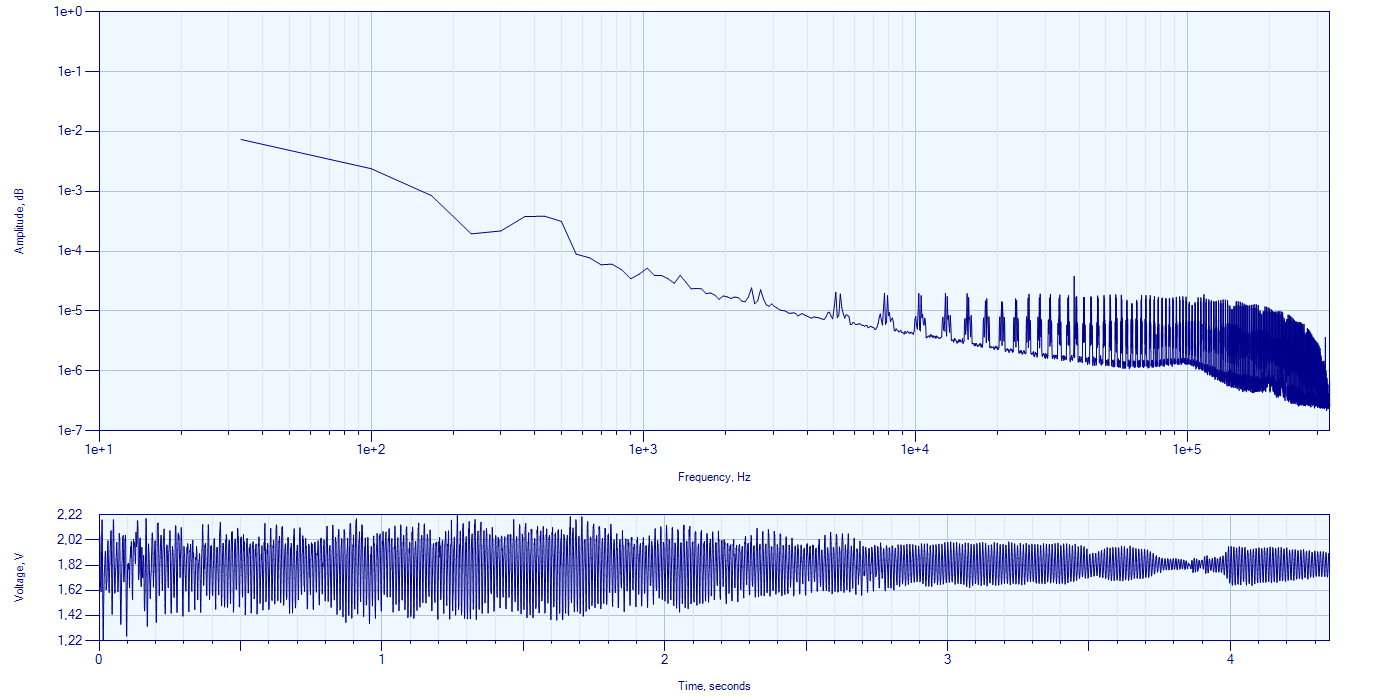
\includegraphics[width=\textwidth]{images/fft-server}
\caption{Изображения, получающиеся при преобразовании Фурье на удаленном CUDA-сервере}
\end{figure}

\end{document}
